\documentclass[12 pt,a4paper,autodetect-engine]{jsarticle}
\usepackage{amsmath}
\usepackage{amssymb}
\usepackage{bm}
\bibliographystyle{junsrt_OB}
\usepackage{cite}
\usepackage{textcomp}
%\usepackage[dvipdfmx]{hyperref}
\usepackage[dvipdfmx]{graphicx}
%\usepackage{pxjahyper}
\columnseprule=0.1mm
%\everymath{\displaystyle}
\usepackage{wrapfig}
\usepackage{comment}
\usepackage{3OB}

\graphicspath{./image}


%提出者の氏名・学籍番号・学年
\author{住野豊}%氏名
\id{15XXXXX} %学籍番号
\acay{3}%学年
%共同実験者の氏名・学籍番号
\collabo{
	\mbox{佐藤一朗(15XXXXX)}, \mbox{田中二朗(15XXXXX)}, \mbox{山田三三郎(15XXXXX)}, \mbox{山本四(15XXXXX)},
	\mbox{山元(15XXXXX)}%共同実験者の名前,学籍番号を必ず書くこと
}

%行った実験題目,回数,日付を忘れずに変更すること
\title{レポートテンプレを作った,えらい大変やった疲れ果てた} %実験の題目
\cycle{5} %何回目の実験か「全角」で記入する(1-10)
\subdate{2024年6月16日}%提出年月日
\exdateone{2024年6月2日}%実験年月日1
\exdatetwo{2024年6月9日}%実験年月日2

\begin{document}
\maketitle
\thispagestyle{empty}
\addtocounter{page}{-1}

\section{はじめに}
とりあえず書く,書く,レポートを書く.綺麗な図を作ることは大事だし,\LaTeX を使えば後から数式の位置を変更することも容易.安心してレポートを書くことに集中できる.但し,文章校正の機能は無い,もしくはeditorに有ったとしてもカスなので,ワードで書いてコピペをしていくのも1つの方法と言える.こうしていけば日本語のミスなどが減る.とは言え,かならず自分で校閲をかける習慣を付けることは大事である.

レポートを作成する際は,まず書くべき事を概ねフローチャートにて手元に書いてみる.この時,ひとまずストーリーの流れを書いてみるのがひどく大事である.フローチャートまで行かなくとも,書くべき事を箇条書きにしておくと,言いたいことが重複無くもれなく書けるのでおすすめである.

その後,実験設定$\rightarrow$実験結果$\rightarrow$考察$\rightarrow$背景の順番に書いていく.決して背景から描き始めないように.時間がかかってしまう\footnote{背景に力を入れたくなる気持ちは分かる.というより,まとまった概念なので気持ちよく書ける.ある種の勉強にもなるから否定はしないけど,やることをやってから書いた方が良いよね.}.出来れば実験が終わって暇があるならそのときに,実験設定$\rightarrow$実験結果の部分は荒く完成させてしまうと良い.どうせ後から手を入れられる.このように,書きやすい場所から書き始められるのはTeXの良いところである.式番号や図の番号は簡単に自動的に変えられるから,ひとまず書いた内容を徐々に良くすることが可能なのである.

なぜTeXを使わないか?コマンドが分からないのでは?という不安もあるが導入が難しいと言うことも敷居の1つであろう.おすすめの組み合わせは,WindowsならばTeXliveを導入し,その後TeX Studioを使うこと.きっとTAも一度は悩んでいるので,TeXの書き方で詰まったら質問してみよう.教員もきっと助けてくれるはず.

Macでの導入は...確かそこまで難しいことは無いが,linuxベースなので自由度が高くて,かえって大変かも.

と,2019年のときは書いていたが、Macを使うようになって気づいたが、brew installでほとんど一撃に近かった. Google先生に Mac tex installでいくらでも入れ方が分かる。

WindowsでもMacでもLinuxでそうだが、2024年現在ではVS Codeが神だ。こいつを入れると代替うまくいく。VS Code tex install WindowsやVScode tex install MacなどでGoogle先生に教えを請おう.だいたいQiitaが引っかかるはず.

最近はOverleaf(\verb|https://www.overleaf.com|)のようにクラウド上で作成も出来る.これも1つの方法であろう.日本語導入に少し手間取る場合もあるが,多分大丈夫やってみるべき.一応,解凍したファイルをすべてアップロードすることで作成できるはずである.微妙にローカルの時とオプションが変わるときがあるので.良く留意すること.

以上の流れだが,困ったらgoogle先生に相談するのは最も大事.同じ悩みを抱えた人が必ずいる.どうしても見つからないときは英文で聞くと100\%いる.人間皆同じ悩みを抱えて生きているのである,
確かにgoogleに検索するだけでは知恵にはならないが,知恵をつける上でgoogleでの検索は有効な手法である.鵜呑みにしないこと,少し疑いつつ批判的な目を持って利用することを意識すれば検索するのも悪くないはずだ.


\subsection{ついでに}\label{tuide}
サブセクションなんてのもある,セクションを分けていきたいときに便利.
こんな感じで見た目がガンガン綺麗になる.嬉しい.

\subsection{こんなことも出来る}
二つ目のsubsectionなんて余裕である.また第\ref{tuide}章で書いたことがあれば,\verb|第\ref{tuide}|章と書くだけですぐに相互引用できる.相互引用の順番が仮に変わっても,全く気にしなくて良い!!これは,長い文章を書き始めると本当に偉大であることが分かる.

\subsubsection{まだある}
サブサブセクションもある,ここまでくるとチョットきてる.分けすぎではないか?っていうかここまで細分化できるの知らなかった.


\section{図表の入れ方}
図は何で作ろうか?ひとまずだれもが持っているのはpower pointだろうから,それを使うのが良いだろう.お金持ちなら\footnote{学生版があるが年間11760円,高いとみるか安いとみるか}Adobe Illustratorに慣れても良いかも,epsファイルを扱えるのが魅力.無料ソフトにこだわるのであればinkscape\footnote{\verb|https://forest.watch.impress.co.jp/library/software/inkscape/|}もあり.チョット癖あり.

power pointで作ると,周りにいらない余白が出来る.この余白を消すのに多大なるコツが必要.多少画像劣化するのを許すのであれば,Irfan View\footnote{\verb|https://forest.watch.impress.co.jp/library/software/irfanview/|}という無料ソフトをいれ,power pointの図をペーストして,その図をjpgファイルにすると取り込める.せっかくのベクター形式で作成しているのに,ビットマップ的なファイルになるのが難点とも言える.

グラフは何で作ろう?gnuplotで作ると格好いいし,非線形関数でのfittingもあっという間に出来る.でもチョット慣れるまで大変なのと,エクセルとの連携は欠かせない.エクセルの図を貼るには,先ほどと同様にIrfan Viewにペーストしてjpgで保存するのが良いのか?私は概ね形式を整えたら,Adobe Illustratorでごまかしている.たまにExcelのグラフもIllustratorにペーストした後手を入れて成形している.ズルだ.

理科大の学生なら,MatlabもMathematicaも使えたはず.それぞれ多少癖があるが良いプロットが作れる.これらのソフトは本当はめちゃめちゃ高い!!PCをもう一台買うのと同等ぐらいしうる.うれしがって自分のPCに入れてしまえば悦に入れる.ただし重たいので容量を圧迫するから要注意.

将来計算機をバンバン使えるようになりたいなら,pythonも1つのチョイス.numpy, scipy, matplotlibを組み合わせれば実質Matlab.しかも今後色々と計算機を学んでいく上で良い一ステップ目になる.とは言えscript言語なので本気で色々数値計算を行うのであれば,併せてCやC++を勉強しましょう.


\begin{figure}[hbt]
	\begin{center}
	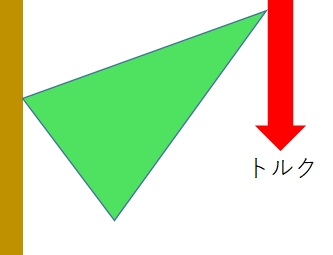
\includegraphics[width=5cm]{test.jpg}
	\caption{図はこのようにして入る.なぜトルクの図なのか?そこら辺にあって使いやすかったからで特に意味は無い.緑色は三角,赤色の矢印は印加した外力に相当している.}
	\end{center}
\end{figure}


\section{数式の作り方}\label{chapter}
\verb|$\int_0^\infty$|と打ち込む,すると$\int_0^\infty$とでる.文章の行に出てくるやつはチョット不細工.

でも,\verb|\[ \int_0^\infty \]|だとこんな感じ\[ \int_0^\infty \].別行に出したいけど,式番号もつけたくない,そんなあなたにお勧め.

式番号をつけたければ
\begin{align}\label{test}
\int_0^\infty
\end{align}
こうして,\verb|\label{test}|として,ラベルを\verb|\begin{align}|の後につけると,
好きなときに式(\verb|\ref{test}|)とするだけで,式(\ref{test})とでる,幸せになる.引用が楽ちんだが,式()の部分は手入力なので注意.

最近知ったのだが,式\verb|\eqref{test}|とするだけで,式\eqref{test}とでる,もはや()を書かなくて良いのだ.ますます幸せになる.

実は\verb|\label{}|は章,図などなど何でも共通である.第\ref{chapter}章,などと記入することも可能.

前は\verb|\begin{align}|ではなく\verb|\begin{equation}|を使っていたが学生に化石と呼ばれて凹んだ.

\section{引用をしよう}
引用文献を本文中で引くことは非常に大事である.例えば,「積分記号を示すには\verb|$\int$|と打ち込む,すると$\int$が表れる\cite{美文書}.」となどと,用いた知識をその場その場で,引用することが重要である.引用は\verb|\cite{}|で指定したbibidを入れてあげるだけで良い.少しわかりにくければソースを見てみよう.これにより読者が議論の詳細に疑問・不明点を感じた際は即座に引用文献を参照することが出来るのである.\verb|\cite{}|と\verb|\ref{}|の役割が若干,違っているので戸惑わないように.

引用の形式にも注意して頂きたい.ここでは\cite{example}を見て欲しい.引用部分に目を移すと,英文の場合,著者はFirst nameはイニシャル,Family nameはフルで書き,複数著者はカンマで区切った後,最終の著者はandでつないでいる.論文誌は斜体,巻号は太字としページ範囲,出版年を記述する.これらは最低限必要な情報であり,太字・斜体の区別や順番は雑誌の規定に応じて前後するが論文中で統一されていることは必須である.概ねここのレポートではテンプレートに統一しておくと良いだろう.

また,bibtexを用いると,更に引用文献の順番も心配しないですむ上,同一のbibファイルを使い回すことが出来る.やや応用物理実験のレポートでは大げさかもしれないが今後研究室に配属されることを考えるのであれば,今慣れておいて損は無い.templateにはbibのスタイルファイルも入れておいた.こちらを使って頂いても結構である.使うときは冒頭で\verb|junsrt_OB.bst|を\verb|\bibliographystyle{junsrt_OB}|で導入すること.

最後に,引用文献や文献値の出典として応用物理学実験の教科書を引用する学生が散見される.しかしながらこれは不適切である.応用物理学実験の教科書は一次資料では無い.文献値に関しても,教科書の値がどのような文献から得られたのかは示されていない.つまり「どういった条件」でその値が得られたかは不明なのである.教科書の引用を良く探し,一次資料を引用することを心がけて欲しい.同じ理由で,本来は理科年表も引用文献としては劣っている.

\section{footnoteも作れる}
脚注が好きなのはなんだか理論家の人に多い気がする.本文の途中で\verb|\footnote|と書いてやると\footnote{こんな感じで下に出る}星が出てしたにゴニョゴニョ書ける.理論家が好きなのは微妙な論理の部分を詰めるのが好きだからでは?との意見もある.あまり脚注が多いと少しかっこ悪いが,使いまくりたくなる気分もよく分かる.

\section{内容が大事}
このようにTexを使うと,内容に集中して書くことが出来る.仮に,後から思い立って内容の順番を入れ替えることも全く恐れる必要は無い.ドンドン書いて素晴らしい考察をしよう.

\section{誰か使ってみませんか?}
こちらのtemplateまだまだ$\beta-2$版です.使ってみてどうなったか知りたいです.またそのとき引っかかった知見をためたいので,これを使ってレポートを書く猛者の人,募集中です.

\begin{thebibliography}{99}
	\bibitem{美文書} 奥村晴彦,黒木裕介『\LaTeXe 美文書作成入門』第7版(技術評論社,2017).
	\bibitem{example} Y. Sumino, I. Sato, J, Tanaka, M, Yamada, Y. Yamamoto and G. Yamazaki {\it Phys. Exp. Tokyo. U. Sci} {\bf 1}, 123-334 (2017).

\end{thebibliography}
\end{document}

